\section{Introduction}
\label{sec:intro}

Facial emotion recognition is a topic of significant relevance and ongoing debate, not only in our daily life, but also in the fields of artificial intelligence and computer vision.
In this short proposal, we aim to leverage several deep neural networks to analyze and interpret different human facial emotions.

The structure of this report is arranged as follows. 
% \Cref{sec:related} contains the related work of our research. 
In~\Cref{sec:datasets}, 
we provide the datasets we used, 
the model architecture we implemented. 
The preliminary evaluation results of our models are given in~\Cref{sec:result}. 
In~\Cref{sec:optim} describes the optimization strategies we have already used and plan to investigate in the coming weeks. 
Finally,
an overview of our time schedule for the entire final project is given in \Cref{fig:schedule}. 
Our code and supplementary material are available at \url{https://github.com/werywjw/SEP-CVDL}.

%-------------------------------------------------------------------------
% All authors will benefit from reading Mermin's description of how to write mathematics:
% \url{http://www.pamitc.org/documents/mermin.pdf}.


% \begin{figure*}
%   \centering
%   \begin{subfigure}{0.68\linewidth}
%     \fbox{\rule{0pt}{2in} \rule{.9\linewidth}{0pt}}
%     \caption{An example of a subfigure.}
%     \label{fig:short-a}
%   \end{subfigure}
%   \hfill
%   \begin{subfigure}{0.28\linewidth}
%     \fbox{\rule{0pt}{2in} \rule{.9\linewidth}{0pt}}
%     \caption{Another example of a subfigure.}
%     \label{fig:short-b}
%   \end{subfigure}
%   \caption{Example of a short caption, which should be centered.}
%   \label{fig:short}
% \end{figure*}

\section{Approach}
\label{sec:approach}

\subsection{Dataset Acquisition and Processing}
\label{sec:datasets}
To initiate the training, 
we acquired the databases FER+\cite{barsoum_training_2016}, RAF-DB\cite{li2019reliable}, CK+\cite{5543262}, TFEID\cite{tfeid} and the videodatabase DISFA\cite{6475933}, from public institutions and GitHub-repositories.
Based on these databases we created a dataset by augmentation to increase variety, 
full details of augmentation is given in \Cref{sec:optim:aug}. 
In terms of the illustrating content of the used pictures, we exclusively used human faces representing 6 emotions. We generalized a folder structure annotating the labels 1 (surprise), 2 (fear), 3 (disgust), 4 (happiness), 5 (sadness), and 6 (anger). 
Beside the original format of images and videos, we set standards for extracting frames from the videos, resizing trainingpictures to 64x64 pixels, saved them as JPEGs.

The first test results in \Cref{fig:result} are aggregated from the database FER+. The images are converted to greyscale with three channels as our original convolutional neural network (CNN) is designed to work with three-channel inputs and add random augmentation. Emotions were assigned tags to each individual picture in a CSV file to facilitate further processing in the model.

\begin{figure}[ht]
  \centering
  % \fbox{\rule{0pt}{2in} \rule{0.9\linewidth}{0pt}}
  % \resizebox{.45\textwidth}{!}{
   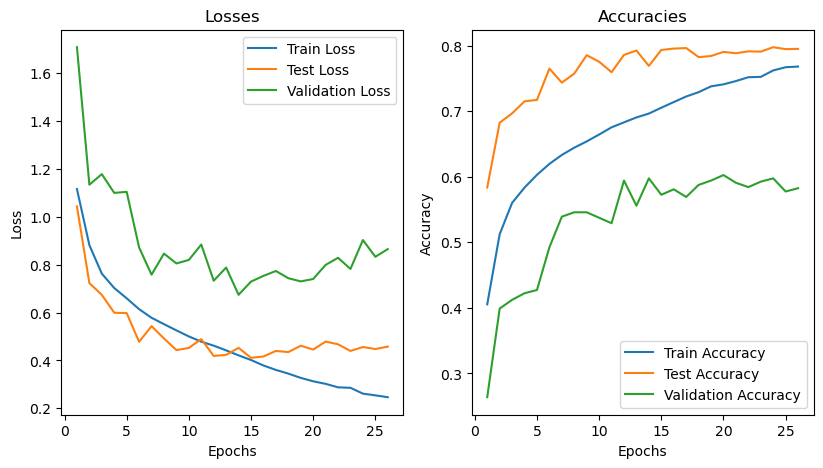
\includegraphics[width=\linewidth]{output.png}
  % }
   \caption{Empirical results in terms of the loss and accuracy on different training epochs}
   \label{fig:result}
\end{figure}

\subsection{Model Architecture}
We implemented from scratch an emotion classification model with four convolution layers at the very beginning. 
Following each convolutional layer, 
batch normalization is applied. 
This stabilizes learning by normalizing the input to each layer. 
Then three linear layers are applied to extract features to the final output. 
We also add a \texttt{dropout} layer to prevent overfitting. 
The activation function used after each layer is Rectified Linear Unit (ReLU), 
since it introduces the non-linearity into the model, 
allowing it to learn more complex patterns. 
In order to find the best hyperparameter configuration (see \Cref{tab:hyper} for details) of the model, 
we utilize the parameter grid from sklearn~\footnote{\url{https://scikit-learn.org/stable/modules/generated/sklearn.model_selection.ParameterGrid.html}}. 

% model comparison, e.g., SVM try, also VGG
% specific dataset comparison, e.g., RAF-DB & FER+
% bold the best results later

\section{Preliminary Results}
\label{sec:result}

For evaluation, we use the metric accuracy. 
As seen in \Cref{tab:model}, 
we report all the training, testing, and validation accuracy in \% to improve the performance of our models. 
The loss function employed for all models is cross-entropy, which is typically for multi-class classification. 
The best results of the performance of the model with respect to loss and accuracy are depicted in \Cref{fig:result}.

\begin{table}
  \centering
  \resizebox{.47\textwidth}{!}{
  \begin{tabular}{@{}lccc@{}}
    \toprule
    Models &  Accuracy (Train) &  Accuracy (Test) & Accuracy (Vali) \\
    \midrule
    CNN (Baseline) & 66.3 & 75.2 & 52.6 \\
    CNN (SE) & 74.3 & 79.9 & 59.6 \\
    CNN (SE-Aug) & 84.6 & 79.5 & 62.8 \\
    CNN (SE+Residual) & 71.5 & 78.9 & 56.4 \\
    ResNet18~\cite{HeZRS16} & 76.8 & 79.8 & 60.3 \\
    \bottomrule
  \end{tabular}
  }
  \caption{Accuracy (\%) for different models in our experiments}
  \label{tab:model}
\end{table}

\begin{table}
    \centering
    \begin{tabular}{@{}lc@{}}
      \toprule
      Hyperparameter & Configuration \\
      \midrule
      Learning rate & \{0.1, 0.01, 0.001, 0.0001\}  \\
      Batch size & \{8, 16, 32, 64\} \\
      Dropout rate & \{0.5\} \\
      Epoch & \{10, 20, 30, 40\} \\
      Early stopping & \{\texttt{True}, \texttt{False}\} \\
      Patience & \{5\} \\
      \bottomrule
    \end{tabular}
    \caption{Explored hyperparameter space for our models}
    \label{tab:hyper}
\end{table}

\section{Optimization Strategies}
\label{sec:optim}
We increase the depth of the network by adding some convolutional layers to learn more complex features. 
We also add the residual connections to help the training of deeper networks more efficiently, 
as they allow gradients to flow through the network more easily, improving the training for deep architectures. 
Moreover, 
we add squeeze and excitation (SE) blocks to apply channel-wise attention. 
In the coming weeks, 
we will focus on the following the tasks~\Cref{sec:optim:aug} and ~\Cref{sec:optim:cam}.
Further research is orientated on papers engaging similar investigations.
\cite{noauthor_multimodal-emotion-recognition00-presentationreportsp4pdf_nodate}, \cite{zeiler_visualizing_2013}, \cite{verma_efficient_2023}, \cite{li_reliable_2017}

\subsection{Augmentation}
\label{sec:optim:aug}
In machine learning and artificial intelligence, 
augmentation stands as a transformative technique, 
empowering algorithms to learn from and adapt to a wider range of data. 
By introducing subtle modifications to existing data points, 
augmentation effectively expands the dataset, 
enabling models to generalize better and achieve enhanced performance.
As models encounter slightly altered versions of familiar data, 
they are forced to make more nuanced and robust predictions. 
With this process we aim to prevent overfitting, 
a common pitfall in machine learning. 
Additionally we guide the training process to enhance recognition and handling of real-world variations.
During the project we pursue various approaches. 
We are implementing different combinations of functions from the \texttt{pytorch.transforms} library and testing already established filters that have been developed, in other research contexts. 
We create various replications of existing photos by randomly altering different properties such as size, brightness, color channels, or perspectives.

\subsection{Explainable AI \& Grad-CAM}
\label{sec:optim:cam}
Class Activation Mapping\cite{zhou_learning_2016} is a visualization technique designed to highlight the regions of an image or video that contribute the most to the prediction of a specific class by a neural network. 
Besides proposing a method to visualize the discriminative regions of a classification-trained convolutional neural network (CNN), the authors also use this method to localize objects without providing the model with any bounding box annotations. The model just learns the classification task with class labels and is then able to localize the object of a specific class in an image. 
CAM provides valuable insights into the decision-making process of deep learning models, like CNNs.
We follow up Grad-CAM\cite{almeida_grad-cam_2023}, introduced as a technique that is easier to implement with different architectures.
This task will be implemented by using the libraris of Pythorch
~\footnote{~\url{https://medium.com/@stepanulyanin/implementing-grad-cam-in-pytorch-ea0937c31e82}}
and OpenCV
~\footnote{~\url{https://opencv.org}}.

\subsection{Table of Classification scores}
\label{sec:optim:csv}
We also wrote a script which takes a folder path as input and iterates through the images inside a subfolder. The output is a csv file representing the corresponding classification scores. 

\begin{figure*}
  \resizebox{\textwidth}{!}{
    \begin{ganttchart}[
      % hgrid,
      vgrid,
      time slot format=isodate,
      x unit=0.3cm, 
      y unit title=0.9cm,
      y unit chart=0.45cm,
      bar height=0.35,
      bar top shift=0.2,
      group right shift=0,
      group top shift=0.1,
      group height=.3,
      group peaks width={0.2},
      milestone left shift=0.5,
      milestone right shift=0.5,
      title label font=\bfseries\Large
  ]{2023-12-21}{2024-02-23}
      \gantttitlecalendar{year, month} \\
      \ganttbar[bar/.append style={fill=LMUGreen}]{Data Collecting \& Processing}{2023-12-21}{2024-01-10} \\
      \ganttbar[bar/.append style={fill=LMUGreen}]{Model Implementing}{2023-12-30}{2024-01-30} \\
      \ganttbar[bar/.append style={fill=LMUGreen}]{Model Training \& Validating}{2023-12-30}{2024-01-30} \\
      \ganttbar[bar/.append style={fill=LMUGreen}]{Report Writing}{2024-01-04}{2024-01-16} \\
      \ganttgroup[bar/.append style={fill=LMUGreen}]{Preliminary Report}{2023-12-21}{2024-01-17} \\
      % \ganttmilestone{Deadline 1}{2024-01-18} \\
      \ganttbar[bar/.append style={fill=Orange}]{Explainable AI}{2024-01-05}{2024-01-30} \\
      \ganttbar[bar/.append style={fill=Orange}]{Model Fine-Tuning}{2024-01-05}{2024-01-30} \\
      \ganttbar[bar/.append style={fill=Orange}]{Video Preparing}{2024-01-17}{2024-02-06} \\
      \ganttbar[bar/.append style={fill=Orange}]{Slides Preparing}{2024-01-20}{2024-02-06} \\
      \ganttgroup[bar/.append style={fill=Orange}]{Presentation}{2024-01-05}{2024-02-07} \\
      % \ganttmilestone{Deadline 2}{2024-02-08} \\
      \ganttbar[bar/.append style={fill=cvprblue}]{Report Writing}{2024-01-17}{2024-02-21} \\
      \ganttgroup[bar/.append style={fill=cvprblue}]{Final Submission}{2024-01-19}{2024-02-22} \\
      % \ganttmilestone{Deadline 3}{2024-02-23}
      % \ganttlink{elem3}{elem8}
      % \ganttlink{elem2}{elem3}
      % \ganttlink{elem2}{elem4}
      % \ganttlink{elem4}{elem5}
  \end{ganttchart}
  }
  \caption{Overview of the schedule for the final project}
  \label{fig:schedule}
\end{figure*}

\subsection*{Author Contributions}
\label{sec:author}
% see https://arxiv.org/pdf/2005.14165.pdf page42
Equal contributions are listed by alphabetical order of surnames. 
Every author did the literature research and contributed to the writing of the paper. 

\begin{itemize}
  \item \textbf{Tanja Jaschkowitz} implemented the model architecture, training and testing infrastructure, and CSV file aggregations. 
  \item \textbf{Leah Kawka} collected the training data, prepared data processing, implemented augmentation, and ran the results. 
  She also takes part in the Explainable AI and Grad-CAM.
  \item \textbf{Mahdi Mohammadi} implemented the augmentation, and did the research searching. 
  \item \textbf{Jiawen Wang} implemented the model architecture, training and testing infrastructure, and optimization strategies. 
  In the specific writing part, she also checked and aggeregated this report from other team members.
\end{itemize}

\section*{Acknowledgements}

We are deeply grateful to our advisors \textbf{Johannes Fischer} and \textbf{Ming Gui} for their helpful and valuable support during the entire semester. 
We also thank \textbf{Prof. Dr. Björn Ommer} for providing this interesting practical course.